\documentclass[conference]{IEEEtran}
\IEEEoverridecommandlockouts
% The preceding line is only needed to identify funding in the first footnote. If that is unneeded, please comment it out.
\usepackage{cite}
\usepackage{amsmath,amssymb,amsfonts}
\usepackage{graphicx}
\usepackage{textcomp}
\usepackage{xcolor}
\usepackage{subfig}
\usepackage{algorithm} 
\usepackage{algpseudocode}
\usepackage{diagbox}
\usepackage{footnote}
\usepackage{bbding} %\Checkmark \XSolid
% to be able to draw some self-contained figs
\usepackage{tikz}
% inlined bib file
\usepackage{filecontents}

\def\BibTeX{{\rm B\kern-.05em{\sc i\kern-.025em b}\kern-.08em
    T\kern-.1667em\lower.7ex\hbox{E}\kern-.125emX}}
\begin{document}

\title{Dynamic Lock Violation for Fault-tolerant Distributed Database System}


\author{\IEEEauthorblockN{Hua Guo}
\IEEEauthorblockA{\textit{School of Information} \\
\textit{Renmin University of China}\\
Beijing, China \\
guohua2016@ruc.edu.cn}
\and
\IEEEauthorblockN{Xuan Zhou}
\IEEEauthorblockA{\textit{School of Data Science And Engineering} \\
\textit{East China Normal University}\\
Shanghai, China \\
xzhou@dase.ecnu.edu.cn}
}

\maketitle

\begin{abstract}
Many modern cloud distributed database management system (DBMS) scale horizontally by sharding its data on many nodes for scalability.
Most of the databases in this category also build their transactional layer upon a replication layer for fault-tolerance.
The replication layer uses a consensus protocol to reach consistency and implement automatic fault recovery.
Many transactions take less time to enforce a serializable schedule than write its commit log to the replicated state machine(RSM). 
Thus,  the replication layer and consensus protocol amplify transactions' lock duration.
Exploit speculative techniques, such as controlled locked violation(CLV) and early lock release(ELR) can shorten lock duration and optimize transaction performance, especially handle a high degree of contention.
However, these techniques, which are mainly focused on single-site database and failed to achieve both performance and correctness on a distributed environment.
In this paper, we introduce dynamic lock violation(DLV) which we designed for the distributed transaction, especially which is on a geo-replication layer for fault-tolerance.
DLV can violate lock at a proper time to get the best performance and achieve both performance and correctness.

\end{abstract}

\begin{IEEEkeywords}
Database System, Distributed Transaction, Locking, High Availability
\end{IEEEkeywords}

\section{Introduction}

Modern distributed
database management system(DBMS)  scale-out by partitioning data into multiple nodes, so it can run transactions on different servers in parallel and increase throughput.
However, when the DBMS needs to access multiple partitions, it uses a coordination protocol to ensure a transaction's atomicity.
Distributed transactions usually lead to significant performance degradation, mainly due to the following reasons\cite{Calvin:conf/sigmod/ThomsonDWRSA12}:

1. Coordinating to commit needs a chatty protocol (i.e., two-phase commit) which causes more message overhead;

2. The message transmission overlaps with the critical path of transaction commit, which worsens the contention among transactions.

Furthermore, distributed DBMS in this category also use a replication layer below the transaction layer to guarantee fault tolerance.
Transactional layer uses a specific concurrency control(CC) scheme to enforce a serializable schedule and a distributed commit protocol if transaction access multiple shards.
%Optimistic CC scales well when there is little contention but suffers high abort rate when it dealing with a workload of high degrees of contention.
%Pessimistic CC has a lower abort rate, but it endures overheads of blocking.
%In fact, CC matters little on performance if no conflicts and no most CC schemes failed to handle high contention\cite{PerformanceOfCC:conf/vldb/CareyS84}\cite{EvaluationOfCC:journals/pvldb/HardingAPS17}.
The replicated layer often uses a Paxos-like consensus protocol to guarantee data replicas consistency.
Typical implementation optimized replication performance by splitting data into very small chunks and build replicated state machines on them.
Although building multiple replicated state machine improve replication performance, it makes distributed transaction even more inevitable,
as distributed transactions can more likely occur on different chunks of data.

\begin{figure}[htbp]
  \centerline{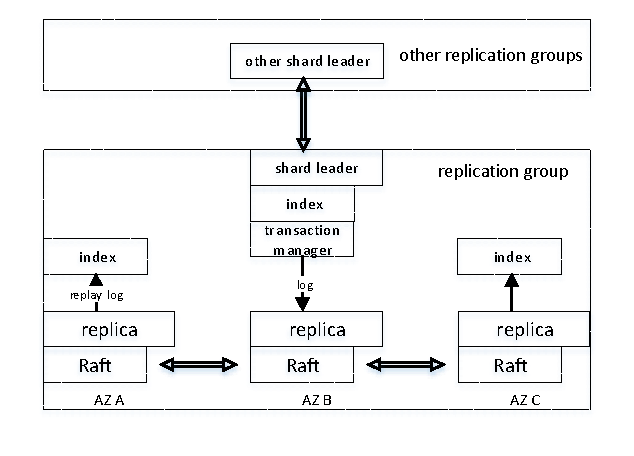
\includegraphics[scale=0.8]{figure/architecture.pdf}}
  \caption{distributed and replicated DBMS Architecture}
  \label{fig:architecture}
\end{figure}

Figure~\ref{fig:architecture} presents the typical architecture.
First, the database partitions its data with many shards to scale.
Second, Each shard works on a replication layer which replicates data in several availability zones(AZ)\cite{Aurora:conf/sigmod/VerbitskiGSCGBM18} for fault tolerance.
Between different available zones, the replication layer uses a consensus protocol to shield consistency.
\begin{figure}[htbp]
  \centerline{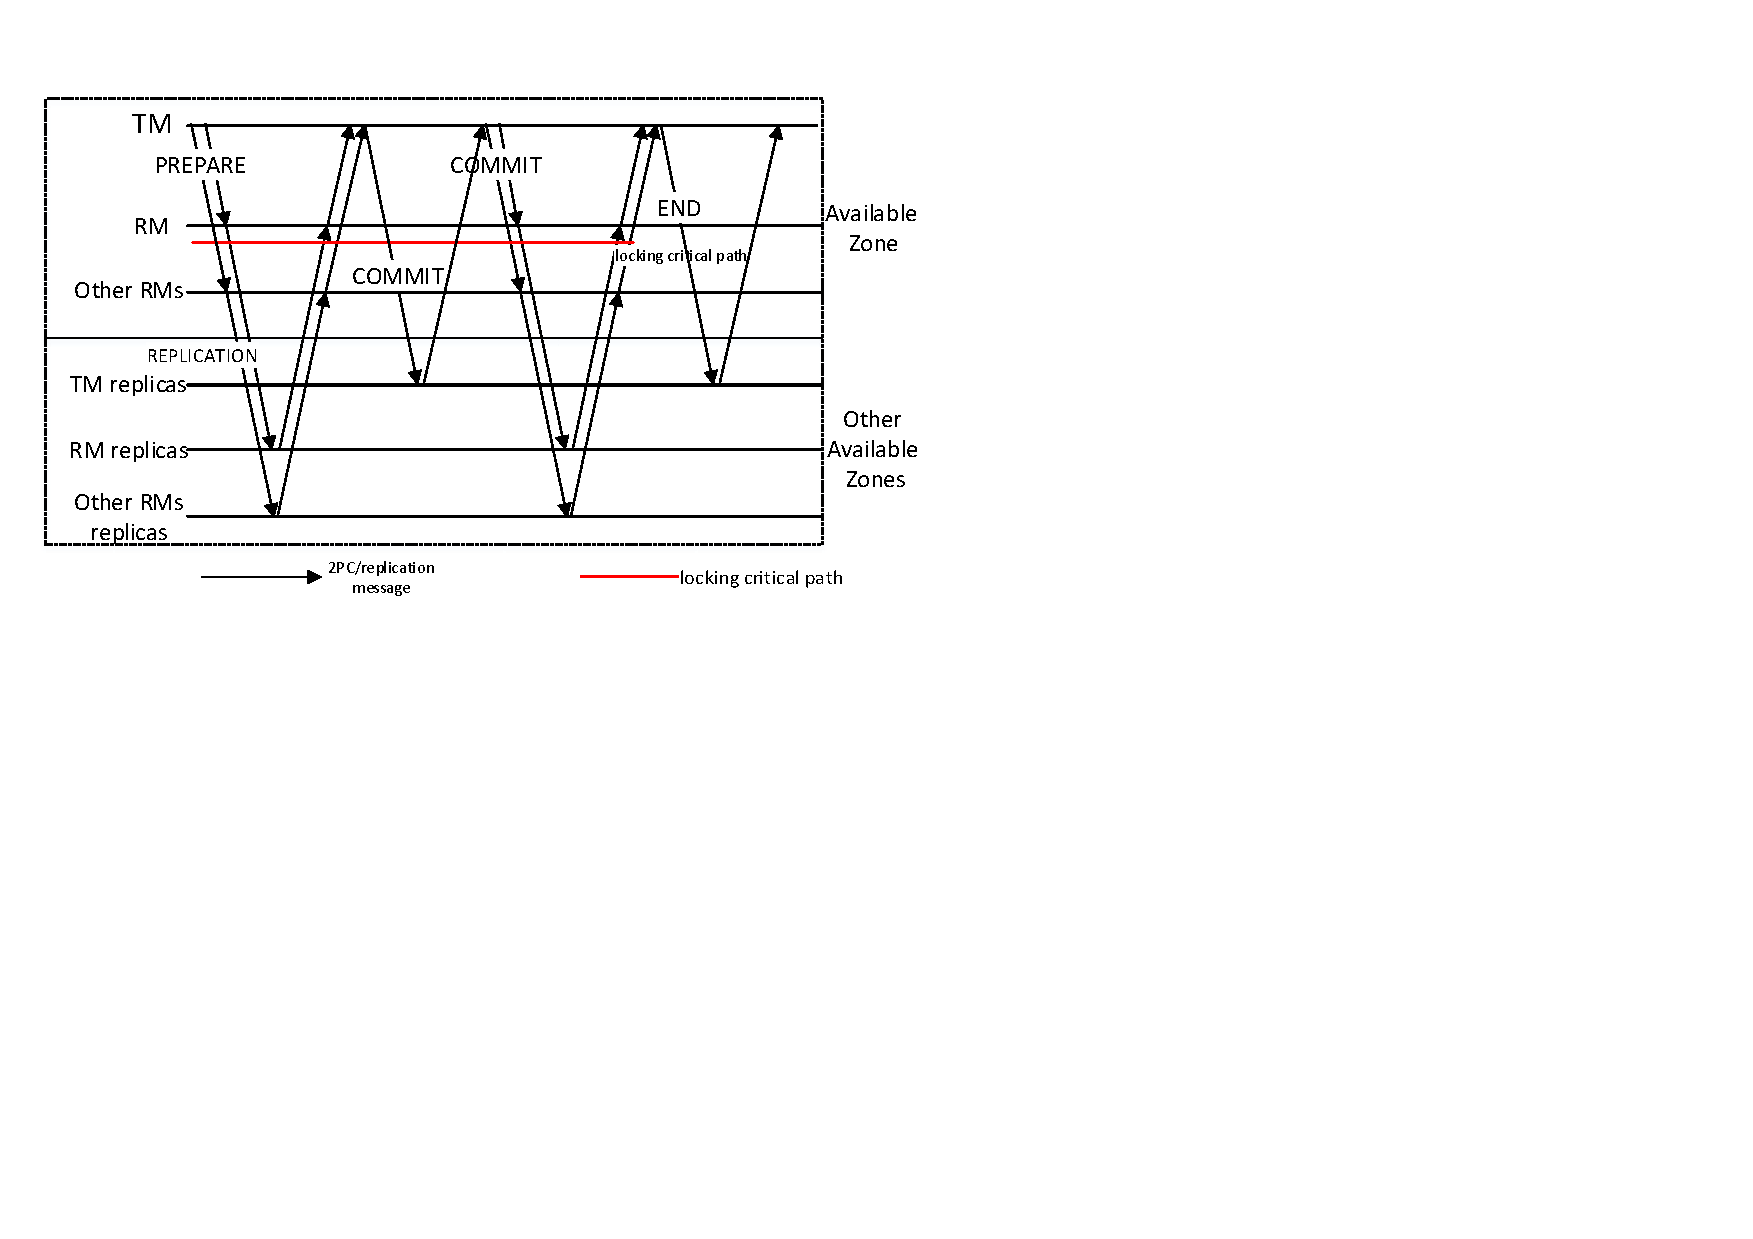
\includegraphics[scale=0.62]{figure/message_flow.pdf}}
  \caption{The message flow and lock hoding critical path of DB who uses 2PL(or with DLV ) and 2PC works on replication layer. 
The dash arrow line message is introduced by DLV. The red lines show the critical path of S2PL and the green dash line shows the critical path of DLV.}
  \label{fig:two_layers_architecture}
\end{figure}
This architecture uses a chatty message protocol fails to scale high contention workload, as much previous work has discussed\cite{Calvin:conf/sigmod/ThomsonDWRSA12}\cite{Tapir:conf/sosp/ZhangSSKP15}\cite{Janus:conf/osdi/MuNLL16}.
But this architecture supports a wide range of transaction models and runs well on many workloads.
Most industry distributed DBMS choose this two-layer architecture, such as Google Spanner\cite{Spanner:conf/osdi/CorbettDEFFFGGHHHKKLLMMNQRRSSTWW12}\cite{Spanner:conf/sigmod/BaconBBCDFFGJKL17}, NuoDB\cite{NuoDB}, CockroachDB\cite{CockroachDB}, TiDB\cite{TiDB}.



The distributed coordination and replication  protocol enlarge the timespan of the critical path and amplified contention cost.
We focus on distributed DBMS which uses locking scheme and coordination protocol on a replicated layer, especially who running transaction processing on geo-replicated layer.
Figure \ref{fig:two_layers_architecture} shows the message flow of a distributed transaction using S2PL and 2PC works on a WAN replication layer.
When a transaction requests its commit, \emph{TM(transaction manager)}  issues a prepare message to each \emph{RM(resource manager}).
\emph{RM} replicates its decision result(prepare commit or prepare abort) to other replicas.
\emph{RM} responses its decision to \emph{TM} after reach a consensus to guarantee fault tolerance. 
\emph{TM} then collects all the \emph{RMs} decisions.
And then it broadcasts the final result(commit or abort) to all \emph{RMs}
\footnote{Depend on varies of implementations, TM can choose to write its log or not.}
.
Once a \emph{RM} receives the final result(commit or abort) from \emph{TM}, it would replicate these result to other replicas.
After the consensus of the commit(or abort) log has reached, \emph{RM} 
can release the locks that it had retained since it first accesses the specified record.

We depict the lock duration with the red line in Figure~\ref{fig:two_layers_architecture} when this transaction commit.
The lock duration covers many message round trips including those over WAN.
Such a commit and replication protocol will severely impair the concurrency when confronted with a high degree of contention.

Previous works used speculative techniques, such as early lock release(ELR) \cite{EfficientLocking:conf/vldb/KimuraGK12}, controlled lock violation (CLV)\cite{CLV:conf/sigmod/GraefeLKTV13} to optimize transaction processing using locking.
These techniques can be extended to a distributed environment to improve concurrency.
The two-layer architecture shares the same bottleneck with single node DBMS on forcing transaction log and faces even worse conditions.
Figure \ref{fig:log_write_latency} shows the log write latency of different environment(TODO... experiments setting).
\begin{figure}[htbp]
  \centerline{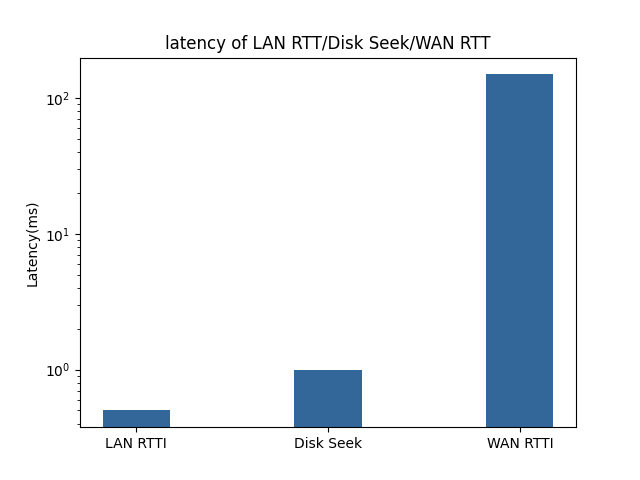
\includegraphics[scale=0.4]{figure/log_write_latency.png}}
  \caption{log write latency in different environment}
  \label{fig:log_write_latency}
\end{figure}

Distributed transactions work on geo-replicated DBMS need more time to write a log than non-distributed and non-replicated one.
However, to apply these techniques on the distributed environment is complex.
There are some design considerations to choose from.
To combine the two-phase commit protocol(2PL), violate(or release) lock at which phase transaction?
As previous work addressed\cite{CLV:conf/sigmod/GraefeLKTV13}, violating lock at the first phase can exploit more concurrency but takes more dependency tracing cost and cascade abort cost.
Violating lock at the second phase need to maintain less dependencies and get less cascade abort rate.
But it may not get better concurrency.
Transaction models, interactive or one-shot transactions, may have different message flow, how different transaction types could benefit from these techniques?
Not all the transactions can benefit from CLV or ELR, little conflicts workloads are such cases.

In this paper, we propose a dynamic lock violation(DLV) to boost the locking-based distributed DBMS, especially who are geo-replicated with a high commit latency.
DLV decides best lock violation time by runtime statistic information.
It maintains less commit dependencies and bears less cascade abort penalty compares previous implementation\cite{CLV:conf/sigmod/GraefeLKTV13}. 

This section is the overall introduction of this paper.
Section \ref{sec:relate_work} is a review of related work.
Section \ref{sec:non_strict} presents a strict schedule is not necessary and hurt the performance of distributed and replicated DBMS.
Section \ref{sec:implement} introduces DLV's implementation.
Section \ref{sec:experiments} evaluates DLV and compare it with previous work.
Section \ref{sec:conclution} draws the final conclusion of this paper.


\section{Relate Work}
\label{sec:relate_work}
This section introduces the related work of this paper.

\subsection{Distributed Transaction on a Replicated Layer}
Recently, there are many scalable DBMS arisen in both academia and industry.
Most of the systems in this category supports distributed query processing and
replicate data across several data center geo-located in different areas for fault tolerance.

A fault-tolerant database relies on state-machine replication(SMR) log to avoid single point failure.
SMR needs to use a consensus protocol to enforce the same order of different replicas.
Paxos\cite{Paxos:journals/tocs/Lamport98}\cite{PaxosSimple:conf/opodis/Lamport02} is the most well-known consensus protocol.
Paxos use two messages round trip to accept a value, one roundtrip for choosing a proposal and another to propose the value.
Multidecree Paxos\cite{Multidecree:journals/csur/RenesseA15} elects a leader as the only proposer to eliminate Paxos first message roundtrip during normal processing.
Raft\cite{Raft:conf/usenix/OngaroO14} is a similar consensus protocol to Paxos, which is designed for understandability.
Consensus introduces significant overhead for its lots of message round trips and heavy network traffic.

Google spanner \cite{Spanner:conf/osdi/CorbettDEFFFGGHHHKKLLMMNQRRSSTWW12}\cite{Spanner:conf/sigmod/BaconBBCDFFGJKL17} is a geo-replicated and shared-nothing DBMS that uses hardware clock for timestamp generation.
VoltDB \cite{VoltDB} is a main memory database who runs single threaded execution per partition.
\cite{Calvin:conf/sigmod/ThomsonDWRSA12} use a deterministic transaction model, 
Calvin can commit distributed transaction without coordination protocol.
VolteDB and Calvin, by using deterministic scheduling, they can use active replication and replicate transaction input rather than transaction effect.
Tapir\cite{Tapir:conf/sosp/ZhangSSKP15} use inconsistent replication layer and build consistent transaction on it to guarantee user level consistent.
Janus\cite{Janus:conf/osdi/MuNLL16} gets fewer wide-area  round trips 
by consolidating the concurrency control and consensus
and use deterministic serializable graph tracing to commit transactions under conflicts.
Tapir and Janus, which benefit from their codesign of transaction and replication layer, can commit a distributed transaction in only one wide-area round trips.

\subsection{Locking Concurrency Control}
DBMS use concurrency control(CC) to calculate a serializable schedule for concurrent transactions.
Two-phase locking(2PL) is the most widely used CC scheme.
As a pessimistic method, 2PL assumes that it is likely that transactions will conflict.
2PL uses a lock to enforce the order of conflicting transactions.
Strict 2PL(S2PL), in additional to 2PL, preserves its lock until a transaction's termination.
S2PL guarantees transaction's recoverability but a 2PL cannot.
For enabling a simple recovery algorithm, most locking based databases choose S2PL.
When extending S2PL to distributed databases, S2PL can take more lock holding time on its commit critical path for many message round trips.

2PL scheme implementation  varies on how they process deadlock.
In \emph{no-wait}
\cite{EvaluationOfCC:journals/pvldb/HardingAPS17}
policy, a transaction would imediantle abort if it fails to lock a record. 
Previous work has proved it is the most scalable technique against other locking schemes, even in diestirbuted environment\cite{EvaluationCC1000Cores:journals/pvldb/YuBPDS14}\cite{EvaluationOfCC:journals/pvldb/HardingAPS17}.
Another policy is \emph{wait-die} \cite{LockNoWait:journals/csur/BernsteinG81} which is similar to \emph{no-wait}.
Transactions avoid false-positive aborting base on their start timestamps when database using 2PL \emph{wait-die}.
In \emph{deadlock detection} \cite{LockCC:conf/ds/GrayLPT76},
transactions can wait for each other without controlling.
The transaction would abort only a deadlock occur.
\emph{Deadlock detection} detect deadlock by explicitly tracing wait-for graph and testing circles.
Many traditional single node database\cite{MySQL}\cite{PostgreSQL} use \emph{deadlock detection} technique because it has no false positive abort. 
Deadlock detection on distributed DBMS  is costly since it requires substantial network messages to identify circles.


\subsection{Exploit Speculation and Lock Violation}
Exploit speculation is not a new invention.
Similar approaches have been introduced by many previous works.
Early lock release (ELR)
\cite{ELR:dewitt_implementation_1984}\cite{PS2PL:conf/icdt/Soisalon-SoininenY95}
\cite{Aether:journals/pvldb/JohnsonPSAA10}
\cite{EfficientLocking:conf/vldb/KimuraGK12}
\cite{Actor-Oriented-DB:conf/icde/Bernstein18}
shares the same idea. 
ELR can release transactions' lock without waiting for commit record flushed to disk.
DeWitt et al.\cite{ELR:dewitt_implementation_1984} firstly described ELR.
Soisalon-Soininen et al.\cite{PS2PL:conf/icdt/Soisalon-SoininenY95} proved that the correctness of ELR.
Johnson et al.\cite{Aether:journals/pvldb/JohnsonPSAA10} and\cite{EfficientLocking:conf/vldb/KimuraGK12} evaluated the performance improvement made by ELR.
Kimura et al.\cite{EfficientLocking:conf/vldb/KimuraGK12}\cite{Aether:journals/pvldb/JohnsonPSAA10} also address the weakness of previous ELR implementation\cite{ELR:dewitt_implementation_1984} can produce wrong results for read-only transactions.
Previous work exploits speculation mostly designed for single machine database system
\cite{PS2PL:conf/icdt/Soisalon-SoininenY95}
\cite{Aether:journals/pvldb/JohnsonPSAA10}
\cite{EfficientLocking:conf/vldb/KimuraGK12}.
Jones et al.\cite{LowOverheadCC:conf/sigmod/JonesAM10} use a restirct transaction model\cite{H-store:journals/pvldb/KallmanKNPRZJMSZHA08} implement sepculation.
Control lock violation(CLV)\cite{CLV:conf/sigmod/GraefeLKTV13} achieve the same performance as ELR but with a simple and general implementation.
CLV can apply to distributed databases and optimize both phases of two-phase commit.
CLV can use a ``register and report approach(RARA)''\cite{HeckatonMVCC:journals/pvldb/LarsonBDFPZ11} to implement its dependency.
RARA work well on a single-site database.
When RARA is used to process a distributed transaction, the dependency tracing may be complex and costly.
Many cascade abort on distributed transaction also carries a performance downgrade.


\section{Beyond Strict Schedule And Lock Violation}
\label{sec:non_strict}

In the following subsections, we descript our preliminaries and assumptions, the basic rule to keep transactions' correctness when violating lock.

\subsection{Preliminaries and Assumptions}
The DBMS shards its data by database primary keys.
Each shard replicates its physiological logs across different AZs for fault-tolerance.
The physiological logs record the row-level write operations of each transaction.
The replicated layer use Raft protocol to maintain consensus of the log order. 
Other replication protocols may also work.
Only the replica leader processes the transactional operations.
Both one-shot and interactive transactions are supported.

Figure \ref{fig:transaction_type} shows the message flow of distributed commit of these two different type of transaction models.
As shown in these figures, The interactive transaction needs more message roundtrips compared to the one-shot one.
These two types of transaction model employ different message flow.
Lock violation can comply with these different transaction models, which we will explain subsequently.

\begin{figure}[htbp]
    \centering
    \captionsetup[subfigure]{oneside,margin={0.3cm,0cm}}
    \subfloat[one-shot transaction, the prepare message is a suggestive one to let the RM issue response commit/abort message ]
        { 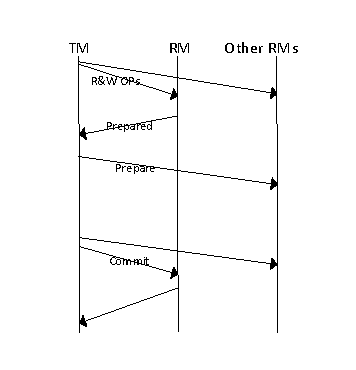
\includegraphics[scale=1] {figure/transaction_oneshot}  \label{fig:transaction_oneshot}  }
    \captionsetup[subfigure]{oneside,margin={0.3cm,0cm}}
    \subfloat[interactive transaction, when a RM receive a \emph{Prepare} message, transaction can prevent deterministic abort. ]
        { 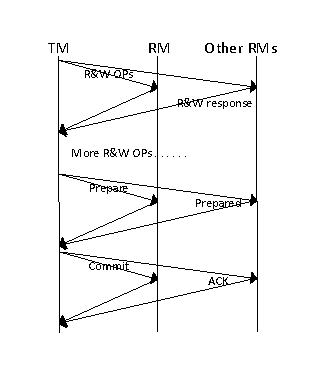
\includegraphics[scale=1]{figure/transaction_interactive} \label{fig:transaction_interactive}}
 
  \caption{commit message flow of one-shot and interactive distributed transaction}
  \label{fig:transaction_type} 
\end{figure}



\subsection{Conceptions and Definitions}
Before we develop our method, we firstly review the formal definition and conception of transaction processing, which can be found in previous work\cite{LockNoWait:journals/csur/BernsteinG81}.

\subsubsection{Distributed Transaction and History}
Given a distributed database has ${n}$
sites ${R = \{r_1, r_2, ... r_n\}}$.
Transaction ${T_i}$ runs on ${m}$ sites  ${S = \{s_1, s_2, ... s_m\} \subseteq R, 1 \le n \le m }$.
Transaction ${T_i}$ runs a series of of operations $o_i$.
$o_i$ can be read or write operation, or command operations which include prepare commit(abort), abort or commit.
${r_i[x]}$ donates transaction ${T_i}$ reads record ${x}$,  ${w_i[x]}$ donates transaction ${T_i}$ writes record ${x}$.
${c_i}$, ${a_i}$, ${p^c_i}$, ${p^a_i}$ mean transaction ${T_i}$ commits, aborts, prepares commit or prepare abort respectively.
We call ${T_i}$'s operations on a site ${s_u}$ as ${T_i}$'s \emph{partial transaction} on ${s_u}$.
The transaction history is a collection ${H = \{h_1, h_2, ..., h_n\}}$,
in which ${h_u (1 \le u \le n) = \Pi_u(H)}$ is the local history on site ${s_u}$.
${\Pi_u(H)}$ is ${H}$'s projection on site ${s_u}$.
For any projected history ${h_u(1 \le u \le m)}$, ${h_{u} }$ is a collection of  operations requests by many transactions.

\subsubsection{Deterministic and Non-deterministic Abort}
Transaction abort due to many reasons, they can be categories:

1. User requested abort, including abort from a user's program logic such as access on non-exists records;

2.Violation of serializability;

3.Database node crash for failure.

We call the first two abort  \emph{deterministic abort} and the last one \emph{non-deterministic abort}.

\subsubsection{Transaction Dependencies}

Transaction ${T_j}$ has a \emph{commit dependency} on transaciton ${T_i}$, written as ${T_j \rightarrow T_i}$, if ${T_j}$ can commit only if ${T_i}$ commit. 
If ${T_j}$ aborts, ${T_j}$ need also abort.
There are there kinds of dependencies, \emph{wr-dependency}, \emph{ww-dependency} and \emph{rw-dependency}.
If in any local history ${h}$, transaction ${T_j}$ read ${T_i}$'s write on ${x}$,
we call this dependency \emph{write-read(wr) dependency} and denote it by ${w_i[x] \rightarrow r_j[x]}$.
Similarly if ${T_j}$ overwrite ${T_i}$'s write on ${x}$, this is \emph{write-write(ww) dependency} and written as ${w_i[x] \rightarrow w_j[x]}$.
And if ${T_i}$ reads ${x}$ is precede ${T_j}$ write on ${x}$ and these two operation has direct conflict(this one seems necessary???), it is a \emph{read-write(rw) dependency} and recorded as ${r_i[x] \rightarrow w_j[x]}$. 
A transaction ${T_j}$ \emph{speculatively access} a record ${x}$, if there is another transaction ${T_i}$, 
${T_j}$ has a dependency on ${T_i}$ and  ${T_i}$ has not committed.
We write this \emph{danger dependency} as ${w_j[x] \rightarrow_s r_i[x]}$, ${w_j[x] \rightarrow_s w_i[x]}$, 
${r_j[x] \rightarrow_s w_i[x]}$.
We also write ${T_j \rightarrow_s T_i}$ to indicate transaction ${T_i}$ has a commit \emph{danger dependency} on ${T_j}$. 

\subsubsection{Strictness}

Traditional transaction schedulers choose strictness\cite{DBLP:conf/vldb/Raz92} to simplify implementation and avoid expensive transaction recovery cost.
Strictness implies that a transaction cannot read or overwrite a previous write by another transaction which has not ended yet.
For a locking base concurrency control scheme, the lock will hold until the transaction end, namely strict two-phase locking(S2PL).
Strictness is not necessary to produce a correct schedule.


\subsection{Strict Scheduler is Too ``Strict" for Correctness}

In schedule ${H_1}$ of Figure \ref{fig:strict_example}, there are 3 transactions working 3 shards, ${s_1}$, ${s_2}$, ${s_3}$.
There are dependencies, ${r_1[x] \rightarrow w_3[x]}$, ${w_1[x] \rightarrow r_2[y]}$, ${r_2[y] \rightarrow w_3[x]}$ and there is ${T_1 \rightarrow T_2 \rightarrow T_3}$.
There is no circle in this dependency graph and the schedule is serializable and strict. 
There is no needs to maintain dependencies explicitly.

Figure~\ref{fig:non_strict_example} shows an example of a non-strict but correct schedule ${H_2}$.
There are three records ${x}$, ${y}$, ${z}$, located at shard ${s_1}$, ${s_2}$, ${s_3}$.
Transaction ${T_1}$ execute write ${y}$, write ${x}$.
Transaction ${T_2}$ read ${T_1}$'s write on ${x}$ before ${T_1}$ commits.
Transaction ${T_3}$ overwrite ${T_2}$'s write ahead ${T_2}$'s commit.
The history 

\begin{center}
  ${H = \{h_1, h_2, h_3\}}$,

\end{center}

in which, 

\begin{center}
  ${h_1=w_1[x]w_3[x]p^c_1c_1p^c_3c_3}$

${h_2=w_1[y]r_2[y]p^c_1c_1p^c_2c_2}$

${h_3=r_2[z]w_3[z]p^c_2c_2p^c_3c_3 }$ 
\end{center}


is not a strict history, but it's a serializable history. 

Both of ${H_1}$ and ${H_2}$ are serializable equal with the serial schedule, ${T_1}$ ${T_2}$ ${T_3}$.
Scheule ${H_1}$ and ${H_2}$ are correct.


\begin{figure}[htbp]
  \centerline{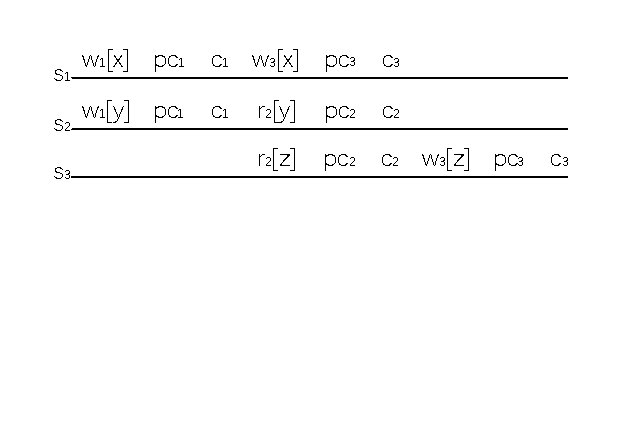
\includegraphics[scale=1]{figure/schedule_strict.pdf}}
  \caption{A strict and serializabile schedule ${H_1}$}
  \label{fig:strict_example}
\end{figure}

\begin{figure}[htbp]
  \centerline{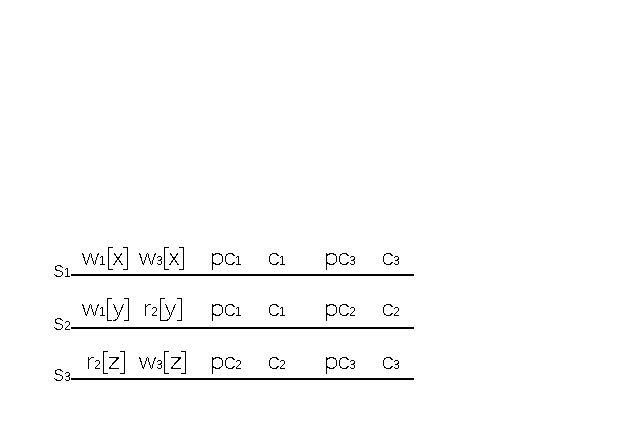
\includegraphics[scale=1]{figure/schedule_non_strict.pdf}}
  \caption{A non-strict but serializabile schedule ${H_2}$}
  \label{fig:non_strict_example}
\end{figure}

\begin{figure}[htbp]
  \centerline{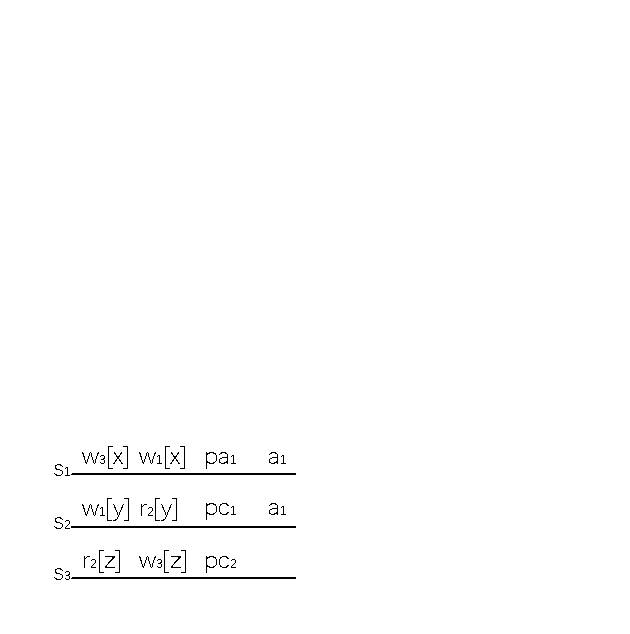
\includegraphics[scale=1]{figure/schedule_not_serializabile.pdf}}
  \caption{Schedule ${H_3}$, ${T_1}$ abort due to non-serializabile}
  \label{fig:schedule_abort_example}
\end{figure}

\begin{figure}[htbp]
  \centerline{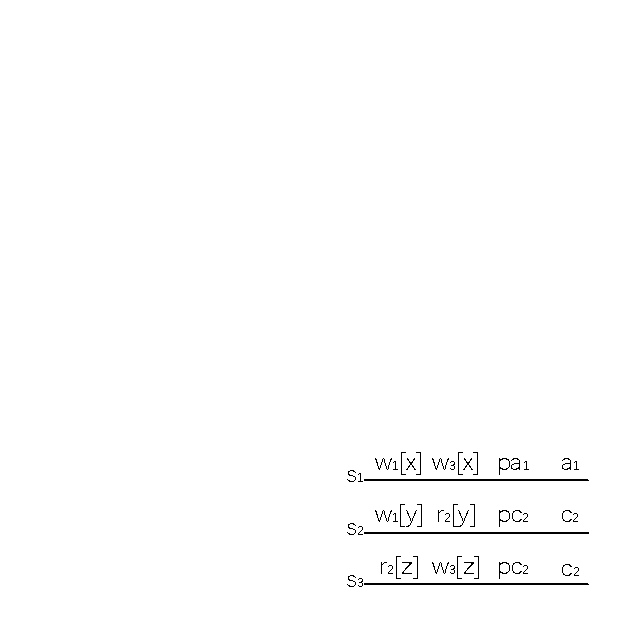
\includegraphics[scale=1]{figure/schedule_not_recoverable.pdf}}
  \caption{Schedule ${H_4}$, ${T_2}$ commit ahead ${T_1}$, non-recoverable anomaly}
  \label{fig:schedule_not_recoverable}
\end{figure}


To get better concurrency, the scheduler can produce schedule like ${H_2}$ in Figure~\ref{fig:non_strict_example}. 
Suppose locking schedule ${H_2}$, then transaction ${T_1}$ must release its locks or make its locks can be violative before it knows its commit decision.
A transaction commits by no means an operation in a flash but progress that needs take lots of time, especially when it is a distributed commit on an RSM.
Strictness scheduler on a distributed and replicated DBMS has a long critical path.
Our basic idea is to develop a serializable but non-strict correct scheduler for distributed transactions and shorten the critical path of committing a transaction.
A single node transaction can exploit log order to maintain logical dependencies because dependent transactions write their logs orderly\cite{ELR:dewitt_implementation_1984}\cite{EfficientLocking:conf/vldb/KimuraGK12}.
When we extended the non-strict locking scheme to distributed transaction, transaction dependency maintaining is more complex.
The serializable scheduler is a correct one if it can prevent abort.
But when there are aborted transactions, it does not.
To produce the correct log, the schedule must be both commit serializable and recoverable\cite{UnifyCR:journals/is/AlonsoVABASW94}.
The scheduler need to maintain commit dependencies to guarantee serializability and recoverability when exploiting non-strictness.

\subsection{Lock Violating Rules and Dependency Tracing}

Lock violation scheduler must follow some rules to preserve correctness.
First, a lock violation scheduler should create serializable schedules.
Consider a schecule ${H_3}$ in Figure \ref{fig:schedule_abort_example} as an example.
There are danger dependencies in ${H_3}$:

\begin{center}
  ${w_3[x] \rightarrow _s w_1[x]}$, 
${w_1[y] \rightarrow _s r_2[y]}$,
${r_2[z] \rightarrow _s w_3[z]}$
\end{center}

There is a circle ${T_1 \rightarrow T_2 \rightarrow T_3 \rightarrow T_1}$.
This schedule is not serializable.
Transaction ${T_2}$
read from uncommitted transaction ${T_3}$.
When ${T_1}$ abort for non-serializable, ${T_2}$ must cascade abort to avoid anomaly.
Assume a lock violation scheduler creates schedule ${H_3}$.
Not formally discussing, a lock violation operation is just as a transaction releases its lock and another later transaction acquire this lock.
Then the schedule ${H_3}$ failed to comply with 2PL's two-phase principle.

For a traditional locking CC scheme, transaction ${T_2}$ needs to wait for ${T_1}$'s release its lock until ${T_1}$ commit.
This situation is like Figure~\ref{fig:strict_example}.
Lock violation scheduler must guarantee the dependency graph has no circles.
A transaction must trace commit dependencies if it violates locks of another conflict transaction operation.

Secondly, a schedule generated by lock violation must also be recoverable.
In schedule ${H_4}$ of Figure~\ref{fig:schedule_not_recoverable}, 
${T_2}$ read from uncommitted transaction ${T_1}$'s write.
There is a danger dependency, ${w_1[y] \rightarrow_s r_2[y]}$ and ${T_2}$ 's commit is ahead ${T_1}$'s commit.
Schedule ${H_4}$ is non-recoverable.
If ${T_1}$ abort, then ${T_2}$ will return an error ${y}$ value.
The scheduler requires to maintain dependencies to preserve the recoverability of the schedule. 


Additionally, there are several design considerations and choices arisen except the correctness.
Can lock violation easily adapt to different transaction models and 2PC?
Violating lock at the first phase of 2PC may be superior to violating lock at the second phase because it can shorten the more critical path length.
But the first phase violation may bear more cascade aborts.
Cascade abort transactions are totally useless work.
DLV permits lock violation at two points in the timeline of running transactions.
We call them \emph{early lock violation} and \emph{late lock violation}.

Suppose ${H}$ is a schedule which is created by lock violation, then ${H}$ is extended by adding the lock, unlock and lock violation operations.
We write ${H}$ by:
\begin{center}
  ${H = l_i[x] o_i[x]... vl_j[x] o_j[x]...  l_i[y] o_i[y]... ul_i[x] ... }$

\end{center}
In ${H}$, ${x}$, ${y}$ are not the same records.
There are following lock/unlock/violation operations,
transaction ${T_i}$ locks record ${x}$;
${T_j}$ violating  ${T_i}$'s lock on ${x}$;
${T_i}$ locks record ${y}$;
${T_i}$ release locks on ${x}$.
If there is such $vl_j[x]$ and $l_i[y]$ operations in schedule ${H}$,
then transaction ${T_j}$ is \emph{eraly lock violate} ${T_i}$'s lock on ${x}$;
otherwise, this is \emph{late lock violation}.
A scheduler uses \emph{early lock violation} may cause non-serializable schedule if it runs without waiting dependencies.
Then DLV needs maintains all $wr$, $ww$ and $rw$ dependencies after violating locks and guarantee the dependency graph of the schedule is acyclic if using \emph{earyly lock violation}. 
On the contrary, \emph{late lock violation} cannot make an acyclic dependency graph to become a cyclic one by adding any dependency edges.
This can be proved by formulating \emph{late lock violation} as 2PL proving.


Assume that there is a \emph{wr-dependency} from ${T_i}$ to ${T_j}$.
    ${T_j}$, which can be written as ${w_i[x] \rightarrow r_j[x]}$.
${T_j}$ cannot commit if ${T_i}$ has not committed.
Traditional S2PL schedule can guarantee this by release locking when ${T_i}$ commit.
Lock violating violates locking rule and ${T_j}$ can read ${T_i}$'s write on ${x}$ before ${T_i}$ commits.
In a lock violation schedule case, transactions must trace dependencies and commit as dependency orders. 
Composite with 2PC protocol, we have the following rules:

\begin{enumerate}
  \item ${T_j}$ prepares only if ${T_i}$ commit;
  \label{rule:prepare}

  \item  ${T_j}$ commits only if ${T_i}$ commit;
  \label{rule:commit} 
  
  \item If ${T_i}$ aborts, ${T_j}$ must also abort

  \label{rule:abort} 
    \end{enumerate}

By tracing dependencies after violating a lock, DLV schedule achieves both serializability and recoverability.

\section{DLV implementation}
\label{sec:implement}

In this section, we introduce DLV implementation. 
The following contents would include:
How DLV can avoid complex recovery algorithm and maintain the most limited amount of dependencies;
How DLV choose the proper time of enabling violation;
The wait-die policy of DLV use;
The pseudocode code description finally.

\subsection {In Memory Speculative Versions}

The non-strict scheduler needs more complex recovery algorithm to keep the correctness.
Take a schedule ${H_5}$ as an example,

\begin{center}
${H_5 = w_1[x]w_1[y]r_2[x]w_2[y]a_1a_2}$
\end{center}

If transaction ${T_1}$ abort, this cause cascade abort for recoverability.
Traditional database use undo log to process recovery transaction write operations.
Implementation undo log maybe a little bit tricky when exploiting non-strict.
A wrong recovery expand schedule of ${T_1}$ may be like ${exp(H_5)}$,
in which ${w^-_i[x]}$ means transaction ${T_i}$ undo its write on ${x}$.

\begin{center}
  ${exp(H_5) =  w_1[x]w_1[y]r_2[x]w_2[y]}$
  ${w^-_1[y]w^-_1[x]c_1w^-_2[y]c_2}$
\end{center}

Suppose the initial value of records ${x}$ and ${v}$ of are both 0. 
The value of records ${x}$, ${y}$ and the undo log formatted after executing every operations in $exp(H)$ is shown in Table~\ref{tbl:x_y_vlues}.
Finally, after the execution of this schedule, both transaction ${T_1}$ and ${T_2}$ aborts.
The value of ${y}$ is 1, which the correct result should be the initial value 0.

\begin{table}[htb]
  \centering
  \begin{tabular}{|c|c|c|c|c|c|}
  \hline
operations & x &  y & undo   \\ 
  \hline
  \hline
  $w_1[x=1]$ & 1 & 0 & x=0  \\ 
  \hline
  $w_1[y=1]$ & 1 & 1 & y=0   \\
  \hline
  $r_2[x]$ & 1 & 1 &    \\
  \hline
  $w_2[y=2]$ & 1 & 2 & y=1  \\
  \hline
  $w^-_1[y=0]$ & 1 & 0 &   \\
  \hline
  $w^-_1[x=0]$ & 0 & 0 &   \\
  \hline

  $c_1$ & 0 & 0 &   \\
  \hline
  $w^-_2[y=1]$ & 0 & 1 &    \\
  \hline
  $c_2$ & 0 & 1 &  \\
  \hline
  \end{tabular}
\caption{x, y values, undo log after the execution of ${exp(H_5)}$}
\label{tbl:x_y_vlues}
\end{table}

To tackle this anomaly, recovery must use a more complex algorithm such as SOT\cite{UnifyCR:journals/is/AlonsoVABASW94}.
For schedule ${H_5}$, a correct recovery expandation may be: 
\begin{center}
${exp^*(H_5) = w_1[x]w_1[y]r_2[x]w_2[y]w^-_2[y]c_2w^-_1[y]w^-_1[x]c_1}$
\end{center}
The schdeuler must recovery transaction by the reserve order of write operation.
If ${x}$ and ${y}$ is on the same database node and use \emph{late lock violation}, the recovery of a transaction is simple.
Because there is no partial failure, the transaction would commit in log order.
No additional work is needed when system recovery using traditional Aries algorithm\cite{ARIES:journals/tods/MohanHLPS92}.

However, if ${x}$ and ${y}$ are not located at the same node, this undo operation order is hard to accomplish because of partial failure.
When using \emph{early lock violation}, there are similar problems since transaction recovery must also undo transactional operations by reserve order.
To avoid this complexity, DLV maintains uncommitted speculative versions in memory and accepts no-steal policy when writing data.
No-steal policy need storage cannot write uncommitted data to permanent storages.
For most transactions would write a little data except the bulk loading ones and the modern database runs on a machine with large RAM, using no-steal policy to save memory is not necessary. 
By no-steal and speculative versions, the database needs no undo log, transaction rollback and failure recovery would be more simple and efficient.
DLV 's speculative version implementation is a little similar with many multi-version concurrency control scheme.
The list is structured from the newest version to the oldest version and the last version of this list is the committed version.
Speculation versions are always stored in main memory and needs no persistence.
If a transaction would abort, it only needs to remove its write versions from speculative version list.

Previously, we have discussed that a \emph{ww} dependency does not affect recoverability.
\emph{Late lock violation}, since it has promised serializability, so it can ignore ${ww}$ and ${rw}$ dependencies and only trace ${wr}$ dependencies for recoverability.
Figure~\ref{fig:versions_example} show a series of schedule access on two contention rows, ${x}$, ${y}$.
The green rectangles are speculative versions and the red ones are committed versions.
Although there is ${ww}$ dependency ${w_6[x] \rightarrow w_4[x]}$.
The abort of $T_4$ does not cause ${T_6}$ cascade abort.
\begin{figure}[htbp]
  \centering
  \captionsetup[subfigure]{margin={0cm,0cm}}
  \subfloat[\small ${H_a = w_1[x_0]w_1[y_0]c_1w_2[x_1]w_3[x_2]w_3[y_1]w_4[x_3]}$]
  { 
    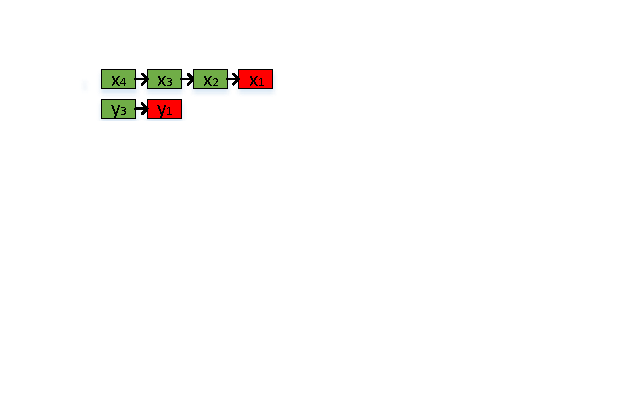
\includegraphics[scale=1.5] {figure/version1} \label{fig:versions_a}}
    \captionsetup[subfigure]{margin={0cm,0cm}
  }
  \subfloat[\small ${H_b = H_a c_2r_5[y_3]r_6[x_4]}$]
  { 
    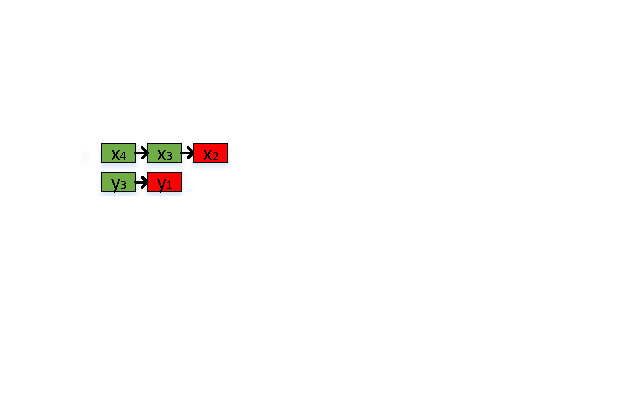
\includegraphics[scale=1.5]{figure/version2} \label{fig:versions_b}
  }
    \captionsetup[subfigure]{margin={0cm,0cm}
  }
  \subfloat[\small ${H_c = H_b a_3a_5}$]
  { 
    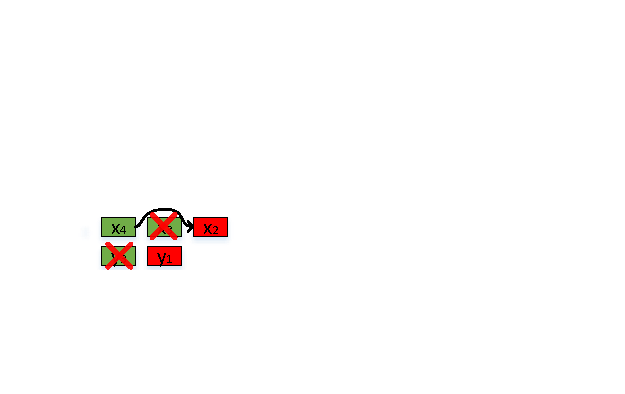
\includegraphics[scale=1.5] {figure/version3} \label{fig:versions_c}}
    \captionsetup[subfigure]{margin={0cm,0cm}}
    \subfloat[\small ${H_d = H_c c_4r_6[y_1]c_6}$]
      { 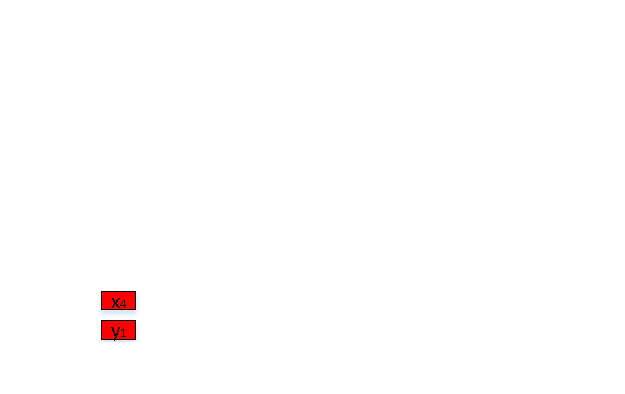
\includegraphics[scale=1.5]{figure/version4} \label{fig:versions_d}
  }
  \caption{speculative(green) and committed(red) versions, 
  ${x_i}$ , ${y_i}$ express this version is from transaction transaction ${T_i}$'s write
}
\label{fig:versions_example}
\end{figure}

\subsection {Dynamic Decide Early or Late Violation}
\emph{Early lock violation} can is more appropriate then \emph{late lock violation} when there are less cascade abort caused by non-deterministic abort.
\emph{Early lock violation} also need more dependency tracing costs.
Too many cascade abort can contributed to a lot of useless work.

We implementation \emph{late lock violation} by adding a message round trip to prevent deterministic abort when use lock violation.
This additional message flow shows in Algorithm~\ref{alg:speculate_phase}.
In Figure~\ref{fig:two_layers_architecture}, the message is show as dotted arrow lines.
Before an ${RM}$ decides to replicate its prepare log, it also sends a \emph{Ready} message to ${TM}$ and tells ${TM}$ it will prepare this transaction.
\emph{Ready} message shows that the ${RM}$ will prepare commit or prepare abort.
When the \emph{TM} collect all \emph{RM}s \emph{Ready} message, it sends \emph{Violate} messages to tells every \emph{RMs} make their locks are violative.
An interactive-transaction can combine these messages with the last operations and prepare requests in passing, as Figure~\ref{fig:transaction_interactive} shows.
So, the interactive transaction needs no dynamic decides the lock violation time.
Interactive transactions use ${DLV}$ would only work as \emph{late violation}.
We mainly focus on discuss one-shot transaction model here.
For a one-shot transaction, this message flow also takes less time than the overall message flow of 2PC because of no log replication time dealy.
Especially when all the ${RMs}$ and the ${TM}$ are located in LAN, there is no WAN message RTT. 

DLV records transaction statistic information to decide use \emph{early lock violateion} or \emph{late lock violation}.
We define a partial transaction which enters prepared commit status but failed to commit finally as partial prepare.
DLV calculates partial prepare rate at a period to decide which violation strategy to choose.
We define that a transaction ${T}$ running at time ${\tau}$ would access a collection of shards
${S_1, S_2, ..., S_n}$. 
The message round trip time(RTT) from ${T}$'s ${TM}$ to ${RM}$ on shard ${S_i}$ is ${RTT_i}$.
In a window period time from ${\tau - \delta}$ to ${\tau}$, there is ${N_p}$ partial preapres of total ${N_t}$ partial transactions. 
DLV would tests the following conditions where ${\Theta}$ is is a constant coefficient. 

\begin{center}
  ${N_p / N_t < \Theta * max(RTT_i), i \in \{1,2, .., n\}}$
\end{center}

DLV would choose \emph{early lock violation} if this conditions satisfied. 
Otherwise, it would use \emph{late lock violation}.


\subsection {Locking Violation and Maintain Commit Dependencies}
DLV use \emph{wait-die} protocol to avoid deadlock.
At the beginning of a transaction, the transaction uses the current timestamp to generate a transaction id.
The conflict transaction operations are queued base their transaction id's order. 


\emph{DLV} use register and report\cite{HeckatonMVCC:journals/pvldb/LarsonBDFPZ11} to maintain dependencies.
Every transaction context stores an in dependency transaction(${in\_dn}$) number count to record how many transactions is the transaction depend on.
The transaction also records an out transaction set(${out\_set}$) attribute record the transactions depend on it.
When a transaction ${T}$ speculative read from ${S}$.
${T}$ registers dependency from ${S}$ by adding ${T}$ to ${out\_set}$ of ${S}$ and increase ${in\_dn}$ of ${T}$ by one.
These steps are described by line 4 - 7 in function READ in Algorithm \ref{alg:execution_phase}.
A transaction cannot prepare if it's ${in\_dn}$ value is greater than 0, which means some in dependency transaction does not commit yet.
If a transaction's ${in\_dn}$ value is less than 0, the transaction must abort because there is some in dependency abort cause a cascade abort.
Algorithm~\ref{alg:prepare_phase} shows how to prepare a transaction.
When a transaction commits, this transaction would traversal its ${out\_set}$ and decrease every transaction's ${in\_dn}$ by one, this is shown in line 6 - 11 of Algorithm \ref{alg:commit_phase} function.
If a transaction aborts, it may cause a cascade abort.
Line 2 of function CASCADE in Algorithm \ref{alg:commit_phase} shows the assign ${in\_dn}$ by a negative value when cascade abort.

\subsection{Pseudocode Description}

Algorithm~\ref{alg:execution_phase} shows the execution phase of a transaction. 
Algorithm~\ref{alg:prepare_phase} shows the prepare phase of a transaction. 
Algorithm~\ref{alg:commit_phase} shows the commit phase of a transaction. 
Algorithm~\ref{alg:speculate_phase} shows the speculation phase of a transaction. 
\begin{algorithm}[!h]

  \caption{Execution phase of transaction ${T}$. Read and write a key}
  
  \begin{algorithmic}[1]
  \Function{Read}{$T,key$}
      \State ${newest\_version \gets Head(Tuple(key).version\_list)}$
      \If {${newest\_version}$ is created by transaction ${S}$ \newline \textbf{and} ${key}$ is ICommit locked by ${S}$ }
        \If {${T \notin S.out\_set }$}
          \State ${S.out\_set \gets S.out\_set \cup T}$
          \State ${T.in\_dn \gets T.in\_dn + 1}$
        \EndIf 
      \EndIf
      \If {${key}$ is \emph{write} locked by transaction ${S}$}
        \State ${S.wait \gets S.wait + 1}$
        \State wait lock till die
        \If {die}
            \State ${T.no\_da \gets }$ \textbf{False}
            \State \textbf{return} die error.
        \EndIf
      \EndIf
      \If {${key}$ is \emph{IAbort} locked by transaction ${S}$}
        \State wait lock this lock released
      \EndIf
      \State Lock(${T, key, Read}$)
      \State \textbf{return} ${key}$'s value.

  \EndFunction
  \label{func:read}
  \end{algorithmic}


  \begin{algorithmic}[1]
  \Function{Write}{$T,key, value$}
    \If {${key}$ is \emph{read} or \emph{write} locked}
      \If {${key}$ is \emph{write} locked by transaction ${S}$}
        \State ${S.wait \gets S.wait + 1}$
      \EndIf
      \State wait lock till die
      \If {die}
        \State ${T.no\_da \gets }$ \textbf{False}
        \State \textbf{return} die error.
      \EndIf
    \EndIf
    \State Lock(${T, key, Write}$)
    \State add a new version of ${key}$'s tuple, assign ${value}$
  \label{func:write}
  \EndFunction
  \end{algorithmic}
  \label{alg:execution_phase}
\end{algorithm}

\begin{algorithm}[!h]
  \caption{Prepare phase of transaction ${T}$}
  \begin{algorithmic}[1]
  \Function{Prepare}{$T$}
    \State wait if ${T.in\_dn > 0}$
    \If {${T.in\_dn < 0}$}
      \State response \emph{TM} message \emph{\{Prepare Abort\}}
    \ElsIf {$T.in\_dn = 0$}
      \State response \emph{TM} message \emph{\{Prepare Commit\}} \newline or \emph{\{Prepare Abort\}}
    \EndIf 
  \EndFunction
  \end{algorithmic}
  \label{alg:prepare_phase}
\end{algorithm}

\begin{algorithm}[!h]
  \caption{Commit phase of transaction ${T}$, commit and (cascade)abort function}
  \begin{algorithmic}[1]
  \Function{Commit}{$T$}
    \State garbage collect old version in \newline ${Tuple(key).version\_list}$
    \For {$ key \in T.write\_set \cup T.read\_set$}
      \State Unlock(${T, key, Read/Write}$)
    \EndFor
    \For {${T_{out} \in T.out\_set}$} 
      \State ${T_{out}.in\_dn \gets T_{out}.in\_dn - 1}$ \Comment{keep exactly once}
      \If ${T_{out}.in\_dn = 0}$ 
        \State report ${T_{out}.in\_dn = 0}$ \Comment{ stop waiting on function PREPARE line 2}
      \EndIf
    \EndFor
    \State response \emph{TM} message \emph{\{Commit ACK\}}
    \label{func:commit}
  \EndFunction
  \end{algorithmic}
  \begin{algorithmic}[1]
  \Function{ABORT}{$T$}
    \State \textbf{call} CASCADE(T)
    \For {$ key \in T.write\_set \cup T.read\_set$}
      \State Unlock(${T, key, Read/Write}$)
    \EndFor
    \State response \emph{TM} message \emph{\{Abort ACK\}}
    \label{func:abort}
  \EndFunction
  \end{algorithmic}
  \begin{algorithmic}[1]
    \Function{CASCADE}{$T$}
      \State ${T.in\_dn \gets -\infty }$
      \For {$ key \in T.write\_set$}
        \If {$key$ is ${ICommit}$ locked by ${T}$}
          \State ModifyLock($T, key, IAbort$)
        \EndIf
        \For {${version \in Tuple(key).version\_list}$}
          \If {${version}$ is created by ${T}$}
            \State remove ${version}$ from list
            \State \textbf{break}
          \EndIf 
        \EndFor
      \EndFor
      \For {${T_{out} \in T.out\_set}$} 
        \State \textbf{call} CASCADE(${T_{out}}$)
      \EndFor
      \label{func:cascade}
    \EndFunction
  \end{algorithmic}
  \label{alg:commit_phase}
\end{algorithm}

\begin{algorithm}[!h]

  \caption{Speculate phase. \
  \newline
  \emph{Ready} and \emph{Speculate} works on \emph{RM}.
  \newline
  \emph{TM} call \emph{Decide} send when \emph{TM} collects all \emph{RM}'s \emph{Ready} message.
  \newline
  \emph{msgs} is a collection of \emph{Ready} message which TM receives from all the \emph{RM}s.
  \newline
  ${\Theta}$ is a threshhold value to enable speculation.}
  \begin{algorithmic}[1]
  \Function{Ready}{$T$}
      \State response \emph{TM} message \newline \emph{\{Ready, ${wait \gets T.wait}$, ${non\_da \gets T.non\_da}$\}}
  \label{func:ready}
  \EndFunction
  \end{algorithmic}
  \begin{algorithmic}[1]
  \Function{Decide}{$T, msgs$}
    \If{${\forall m \in msgs}$, ${m.non\_da}$ is \textbf{True} \textbf{and} \newline
    ${\exists m \in msgs}$, ${m.wait > \Theta}$ }
      \State send all \emph{RM}s message \emph{\{Speculate\}} 
    \EndIf
  \label{func:decide}
  \EndFunction
  \end{algorithmic}
  \begin{algorithmic}[1]
  \Function{Speculate}{$T$}
    \For {$ key \in T.read\_set$}
      \State Unlock($T, key, Read$)
    \EndFor
    \For {$ key \in T.write\_set$}
      \If {$key$ is ${Write}$ locked by ${T}$}
        \State ModifyLock($T, key, ICommit$)
      \EndIf
    \EndFor
  \label{func:speculate}
  \EndFunction
  \end{algorithmic}
  \label{alg:speculate_phase}
\end{algorithm}

\section{Experiments and Evaluations}
\label{sec:experiments}
We develop a replicated distributed DBMS demo and evaluate the performance of \emph{DLV}.
As a comparison with \emph{DLV}, we also implement S2PL wait die(S2PL) scheme, CLV optimize both violate at the 1st phase(CLV1P) and 2nd phase(CLV2P).

\subsection{Experiments Setting}
Our experiments performed on a cluster of 12 Aliyun ecs.g6.large server.
Each server has 2 virtual CPU with 2.5GHz clock speed, 8GB RAM, runs Ubuntu 18.04.
The data is partitioned by 4 shards, each shard has 3 replicas which is replicated across 3 AZs, which is located at Heyuan, Hangzhou and Huhehot.
Every AZ has a full data copy of each shard.
The internal network bandwidth of each AZ is 1Gbps.
We choose a modifies version TPCC and YCSB workload.
All the transactions are distributed transactions.
The TPCC data is sharded by the warehouse id.
The Item table is replicated to all shards.
Each transaction will retry after 3 seconds if it aborts for violation serializability.
The evaluation both tested on both scattered (leader) mode and gathered (leader) mode.
In gathered mode, all of the replica leaders are located in the same AZes.
In scattered mode, the replica leaders are not located in the same AZes.

\subsection{TPCC Performance Evaluation}
Figure \ref{fig:new_order_add_terminal_gathered} shows the NewOrder performance of when adding terminal numbers of each node in the gathered  mode and scattered mode.

Figure \ref{fig:new_order_add_warehouse_gathered},
Figure \ref{fig:payment_add_warehouse_gathered} shows 
the performance of different warehouse numbers.


\begin{figure}[htbp]
  \centering
  \captionsetup[subfigure]{margin={0cm,0cm}}
  \subfloat[NewOrder TPM]
      { 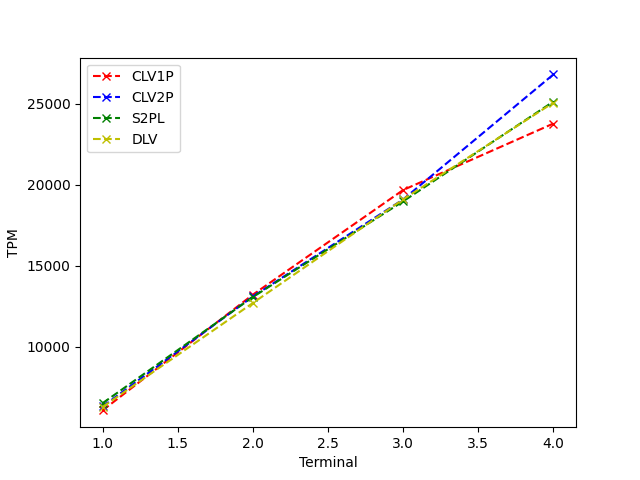
\includegraphics[scale=0.25] {figure/plot_tpcc_neworder_add_Terminal_gather_tpm} \label{fig:new_order_add_terminal_gathered:tpm}}
  \captionsetup[subfigure]{margin={0cm,0cm}}
  \subfloat[NewOrder abort]
      { 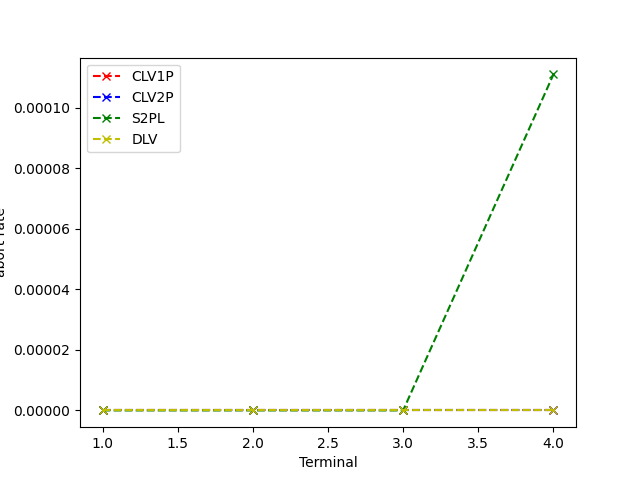
\includegraphics[scale=0.25]{figure/plot_tpcc_neworder_add_Terminal_gather_abort} \label{fig:new_order_add_terminal_gathered:abort}}
  \captionsetup[subfigure]{margin={0cm,0cm}}
\caption{throughput and abort rate of
different terminal number of each node
when running TPCC NewOrder transactions in gathered mode(TODO .. need more terminals, 4 is too small)}
\label{fig:new_order_add_terminal_gathered}
\end{figure}


\begin{figure}[htbp]
  \centering
  \captionsetup[subfigure]{margin={0cm,0cm}}
  \subfloat[NewOrder TPM]
      { 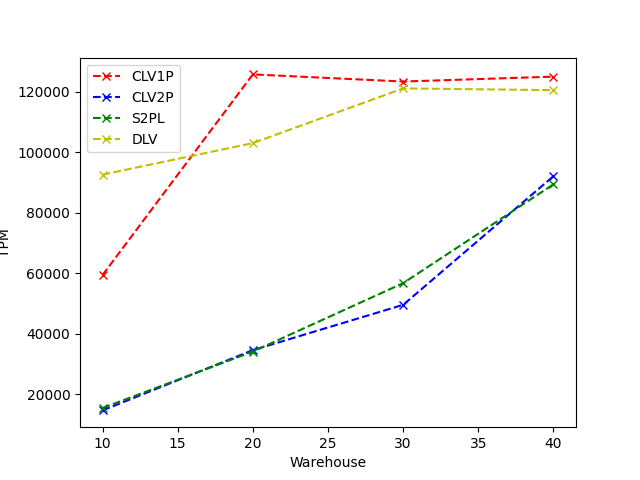
\includegraphics[scale=0.25] {figure/plot_tpcc_neworder_add_Warehouse_gather_tpm} \label{fig:new_order_add_warehouse_gathered:tpm}}
  \captionsetup[subfigure]{margin={0cm,0cm}}
  \subfloat[NewOrder abort]
      { 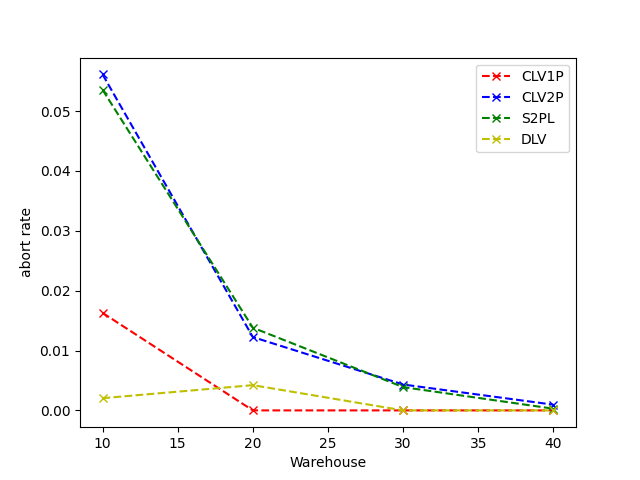
\includegraphics[scale=0.25]{figure/plot_tpcc_neworder_add_Warehouse_gather_abort} \label{fig:new_order_add_warehouse_gathered:abort}}
  \captionsetup[subfigure]{margin={0cm,0cm}}
\caption{throughput and abort rate of
different warehouse number
when running TPCC NewOrder transactions in gathered mode}
\label{fig:new_order_add_warehouse_gathered}
\end{figure}

\begin{figure}[htbp]
  \centering
  \captionsetup[subfigure]{margin={0cm,0cm}}
  \subfloat[Payment TPM]
      { 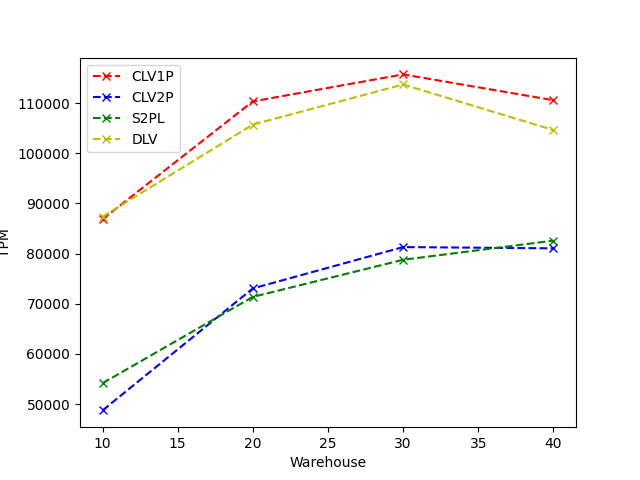
\includegraphics[scale=0.25] {figure/plot_tpcc_payment_add_Warehouse_gather_tpm} \label{fig:payment_add_warehouse_gathered:tpm}}
  \captionsetup[subfigure]{margin={0cm,0cm}}
  \subfloat[Payment abort]
      { 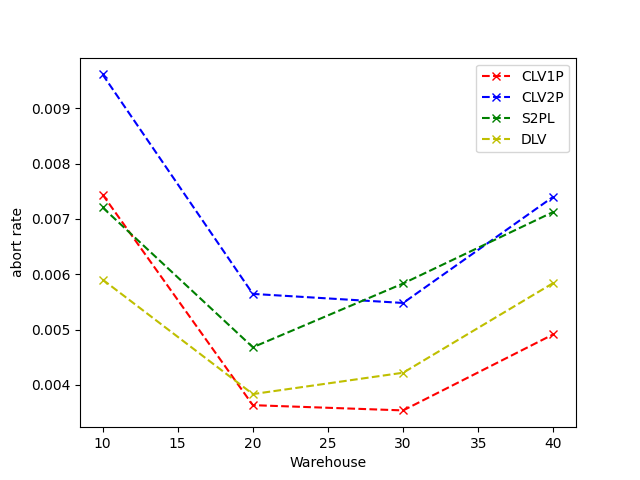
\includegraphics[scale=0.25]{figure/plot_tpcc_payment_add_Warehouse_gather_abort} \label{fig:payment_add_warehouse_gathered:abort}}
  \captionsetup[subfigure]{margin={0cm,0cm}}
\caption{throughput and abort rate of
different warehouse number
when running TPCC Payment transactions in gathered mode}
\label{fig:payment_add_warehouse_gathered}
\end{figure}



\begin{figure}[htbp]
  \centering
  \captionsetup[subfigure]{margin={0cm,0cm}}
  \subfloat[NewOrder TPM]
      { 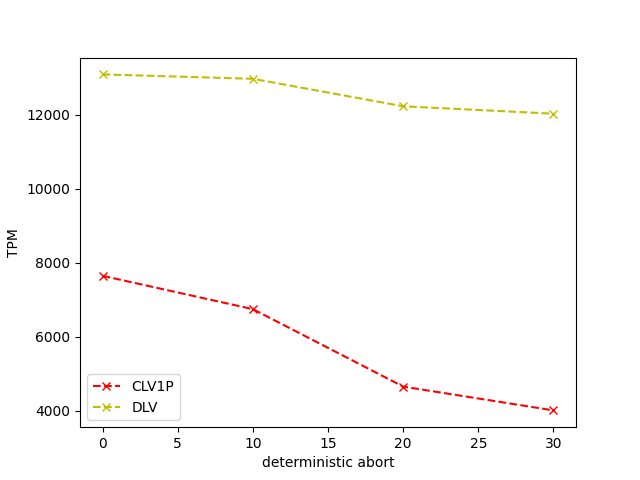
\includegraphics[scale=0.25] {figure/plot_tpcc_neworder_add_NonExist_gather_tpm} \label{fig:plot_tpcc_neworder_add_NonExist_gather_abort:tpm}}
  \captionsetup[subfigure]{margin={0cm,0cm}}
  \subfloat[NewOrder abort]
      { 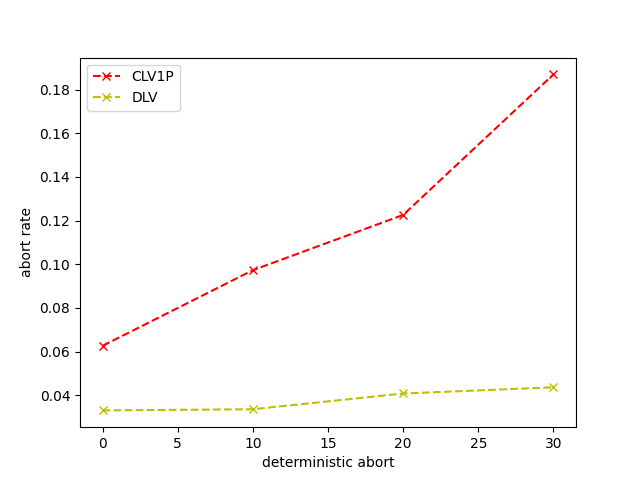
\includegraphics[scale=0.25]{figure/plot_tpcc_neworder_add_NonExist_gather_abort} \label{fig:plot_tpcc_neworder_add_NonExist_gather_abort:abort}}
  \captionsetup[subfigure]{margin={0cm,0cm}}
\caption{throughput and abort rate of
different possible cascade abort rate, 
when running TPCC NewOrder transactions in gathered mode}
\label{fig:plot_tpcc_neworder_add_NonExist_gather_abort}
\end{figure}



\begin{figure}[htbp]
  \centering
  \captionsetup[subfigure]{margin={0cm,0cm}}
  \subfloat[NewOrder TPM]
      { 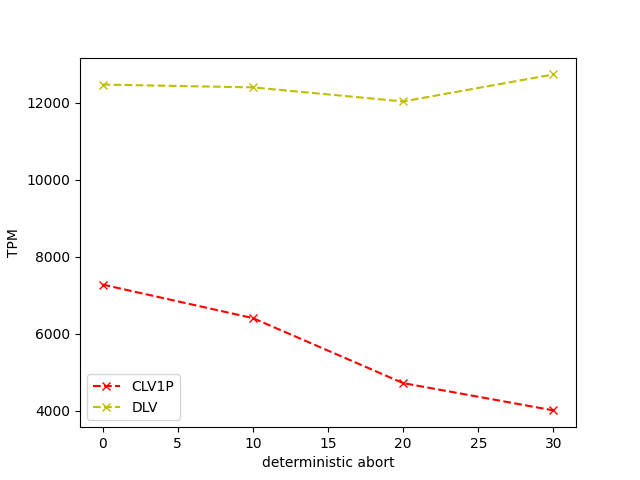
\includegraphics[scale=0.25] {figure/plot_tpcc_neworder_add_NonExist_scatter_tpm} \label{fig:plot_tpcc_neworder_add_NonExist_scatter:tpm}}
  \captionsetup[subfigure]{margin={0cm,0cm}}
  \subfloat[NewOrder abort]
      { 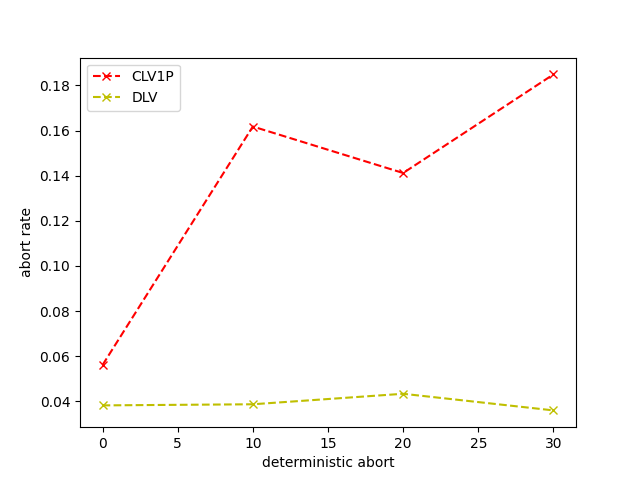
\includegraphics[scale=0.25]{figure/plot_tpcc_neworder_add_NonExist_scatter_abort} \label{fig:plot_tpcc_neworder_add_NonExist_scatter:abort}}
  \captionsetup[subfigure]{margin={0cm,0cm}}
\caption{throughput and abort rate of
different possible cascade abort rate, 
when running TPCC NewOrder transactions in scattered mode
}
\label{fig:plot_tpcc_neworder_add_NonExist_scatter}
\end{figure}

\subsection{YCSB Performance Evaluation}

\begin{figure}[htbp]
  \centering
  \captionsetup[subfigure]{margin={0cm,0cm}}
  \subfloat[YCSB TPM]
      { 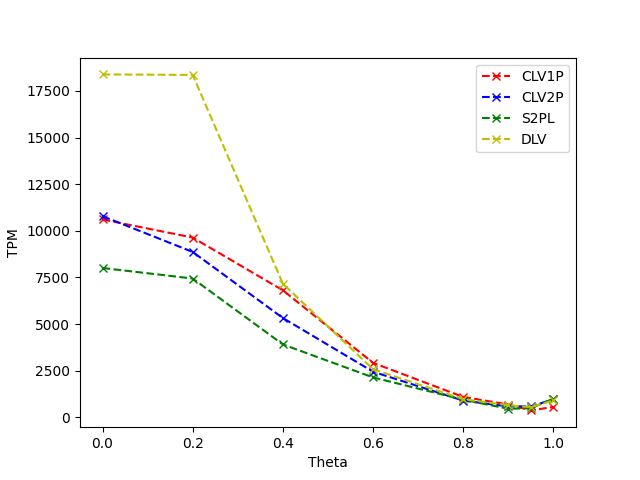
\includegraphics[scale=0.25] {figure/plot_ycsb_add_Theta_gather_tpm} \label{fig:ycsb_add_theta_gathered:tpm}}
  \captionsetup[subfigure]{margin={0cm,0cm}}
  \subfloat[YCSB abort]
      { 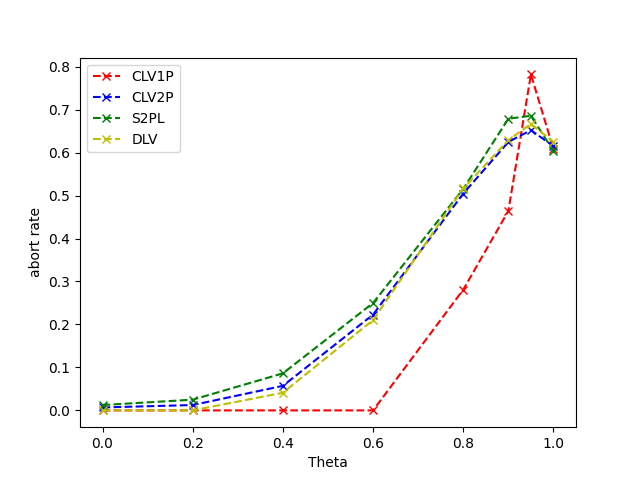
\includegraphics[scale=0.25]{figure/plot_ycsb_add_Theta_gather_abort} \label{fig:ycsb_add_theta_gathered:abort}}
  \captionsetup[subfigure]{margin={0cm,0cm}}
\caption{throughput and abort rate of
different warehouse number
when running YCSB transactions in gathered mode}
\label{fig:ycsb_add_theta_gathered}
\end{figure}

\begin{figure}[htbp]
  \centering
  \captionsetup[subfigure]{margin={0cm,0cm}}
  \subfloat[YCSB TPM]
      { 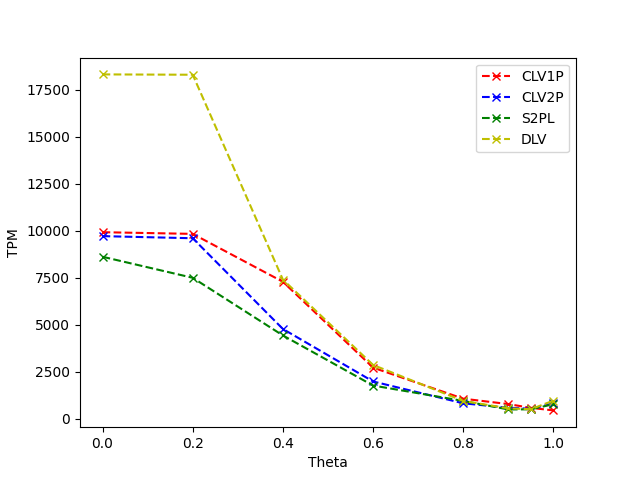
\includegraphics[scale=0.25] {figure/plot_ycsb_add_Theta_scatter_tpm} \label{fig:ycsb_add_theta_scattered:tpm}}
  \captionsetup[subfigure]{margin={0cm,0cm}}
  \subfloat[YCSB abort]
      { 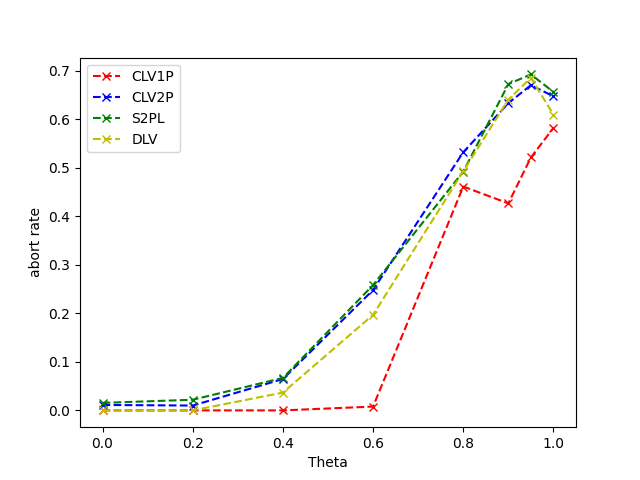
\includegraphics[scale=0.25]{figure/plot_ycsb_add_Theta_scatter_abort} \label{fig:ycsb_add_theta_scattered:abort}}
  \captionsetup[subfigure]{margin={0cm,0cm}}
\caption{throughput and abort rate of
different warehouse number
when running YCSB transactions in scattered mode}
\label{fig:ycsb_add_theta_scattered}
\end{figure}



\section{Conclution}
\label{sec:conclution}
We extend $CLV$ to distributed transaction and evaluate its performance on a geo-replicated environment.
Our distributed version ${CLV}$, i.e. ${DLV}$, can dynamically decide to violate lock at the most suitable time.
${DLV}$ merge many discrete waits at transaction running time into one final wait when commit.
According to our evaluation, ${DLV}$ can improve performance of contention workload for shortening critical path.
${DLV}$ can adapt to different workloads.
It minimize unnecessary dependency tracing cost and cascade abort penalty against previous work.






\bibliographystyle{reference/IEEEtran}
\bibliography{reference/IEEEexample}


\end{document}

